\documentclass[12pt]{article}
\usepackage[left=1in,top=1in,right=1in,bottom=1in]{geometry}
\usepackage{graphicx}
\usepackage{titling}
\usepackage[bookmarks=true,colorlinks=true, linkcolor=red, citecolor=cyan]{hyperref}

\setlength{\droptitle}{-1.0in}   % This is your set screw


\begin{document}


\title{OPL Manual}
\author{Ryan Wisnesky}
\date{\today}

\maketitle

\vspace{-0.5in}

\begin{footnotesize}
\tableofcontents
\end{footnotesize}
\newpage

\section{Introduction}

OPL (Operad Programming Language), a successor to FQL (Functorial Query Language), implements {\it functorial data migration}.  OPL is a language mode within the FQL++/FPQL/OPL IDE, an open-source java program that provides a code editor for and visual representation of FQL++, FPQL, and OPL programs.  A screen shot of the initial screen of the IDE is shown below.  As OPL succeeds FQL, readers are recommended to first familiarize themselves with FQL and the FQL IDE.  OPL also succeeds FQL++ and FPQL, but familiarity with FQL++ and FPQL is not necessary to understand this manual.

\begin{center}
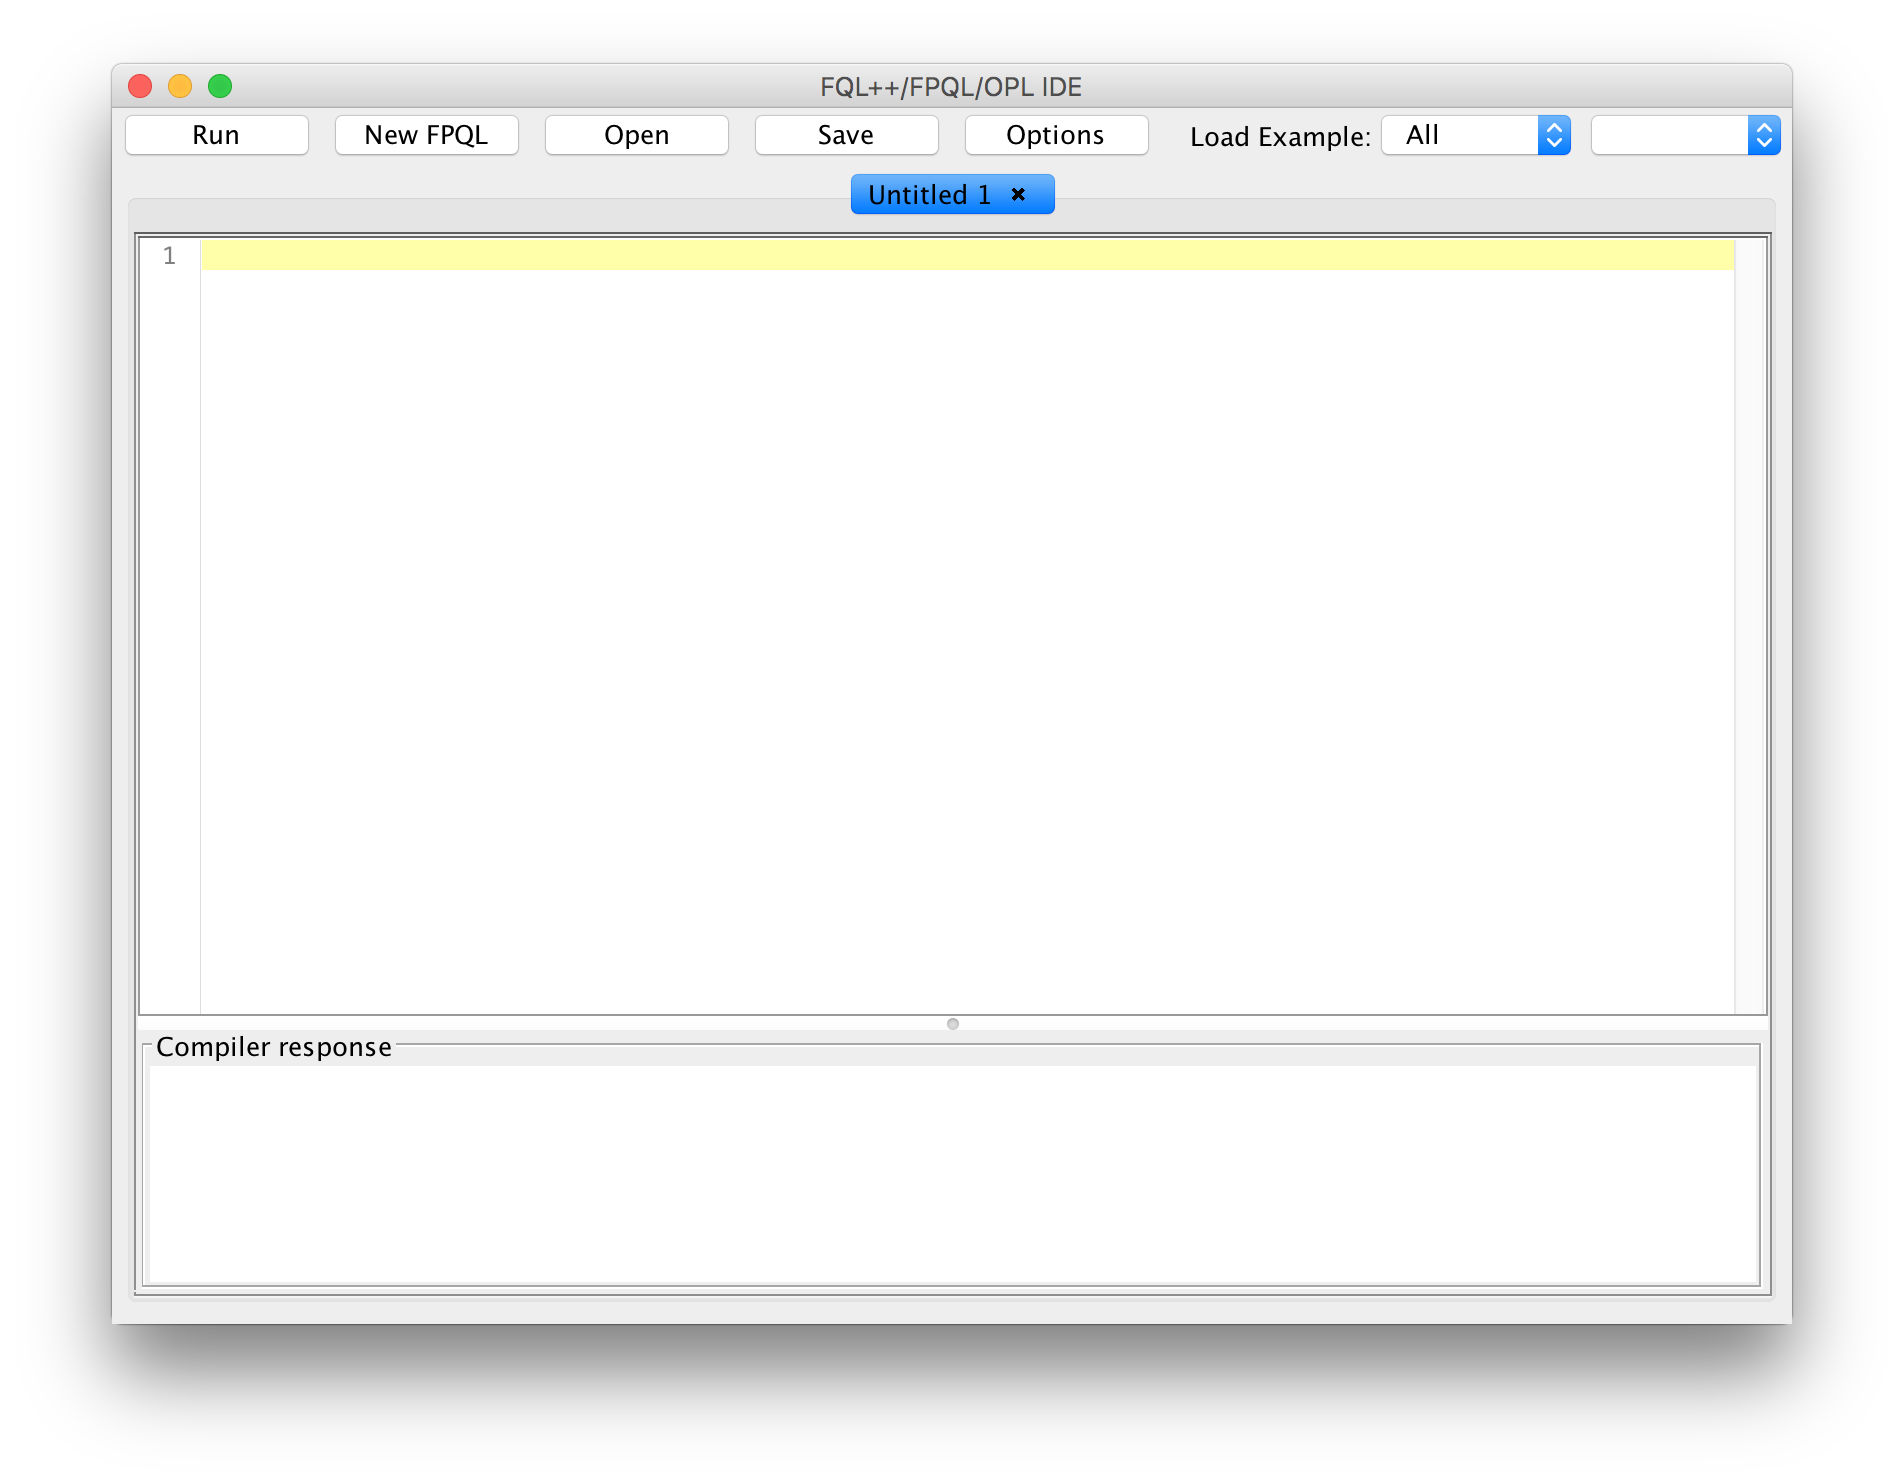
\includegraphics[width=5in]{initial}
\end{center}

The IDE is a multi-tabbed text file editor that supports saving, opening, copy-paste, etc.  Associated with each editor is a ``compiler response'' text area that displays an error message if execution fails.  The built-in examples can be loaded by selecting them from the ``load example'' combo box in the upper-right.  OPL examples are prefixed with ``O'', FPQL examples are prefixed with ``P'', and FQL++ examples have no prefix.  In the rest of this tutorial we will refer to these OPL examples.  Compilation can be aborted with the ``abort'' button in the Tools menu.  Abort is ``best effort'' and can leave the IDE in an inconsistent state; it is provided to allow users to terminate the IDE without needing to invoke the operating system.  

To run the IDE with more than the default 64mb heap, you must use command line options, for example, to specify a 512MB minimum and 2GB maximum heap size, use:
\begin{verbatim}
java -Xms512m -Xmx2048m -jar fql_lib.jar
\end{verbatim}

\newpage

\section{OPL Basics}

Unlike FQL, which focuses on SQL compatibility, the focus of OPL is on integrating the functorial data model with general-purpose programming abilities.  The core concepts in OPL are {\it multi-sorted equational theories} (hereafter referred to simply as theories), {\it mappings} between theories, Set and Javascript-valued {\it models} of theories, {\it finite presentations} of models, {\it transforms} between models and presentations, and {\it queries} over models.  Categorically, theories denote cartesian operads, mappings denote cartesian operad functors, models are Set and Javascript valued functors, finite presentations of models are finite presentations of Set-valued functors, transforms are natural transformations, and queries are compositions of $\Delta$, $\Sigma$, and $\Pi$ data migration functors.  In addition, OPL provides ``typed'' versions of these concepts, which will be discussed in the next section. 
 
An OPL program is an ordered list of uniquely named {\it declarations} of these various kinds.  Comments in OPL are Java style, either ``//'' or ``/* */''. Negative integers must be quoted with double quotes.  Quotes can extend over multiple lines, although syntax highlighting may fail.  A non-negative numeral, such as $0$ or $2$, when used in a place where an OPL expression is required, will automatically convert into an expression involving $zero$ and $succ$; for example, $0$ abbreviates $zero$ and $2$ abbreviates $succ(succ(zero))$.

\subsection{Theories}

Select the ``O KB'' example.  This will create a new tab containing the following OPL code:
\begin{verbatim}
Group = theory {
 sorts 
	S;
 symbols
	e : S,
	I : S -> S,
	o : S,S -> S;
 equations
	forall x. o(e(),x) = x,
	forall x. o(I(x),x) = e(),
	forall x, y, z. o(o(x,y),z)=o(x,o(y,z));
}
\end{verbatim}
This declaration defines a theory $Group$ consisting of one {\it sort}, $S$, three {\it function symbols}, $e$ (of arity 0), $I$ (of arity 1), and $o$ (of arity 2), and three universally quantified {\it equations}.  This is indeed an axiomatization of the free group on zero generators, where $e$ represents the identity element, $I$ represents the inverse operation, and $o$ represents composition.  Press ``run'', select $Group$ from the viewer, and click on "KB":

\begin{center}
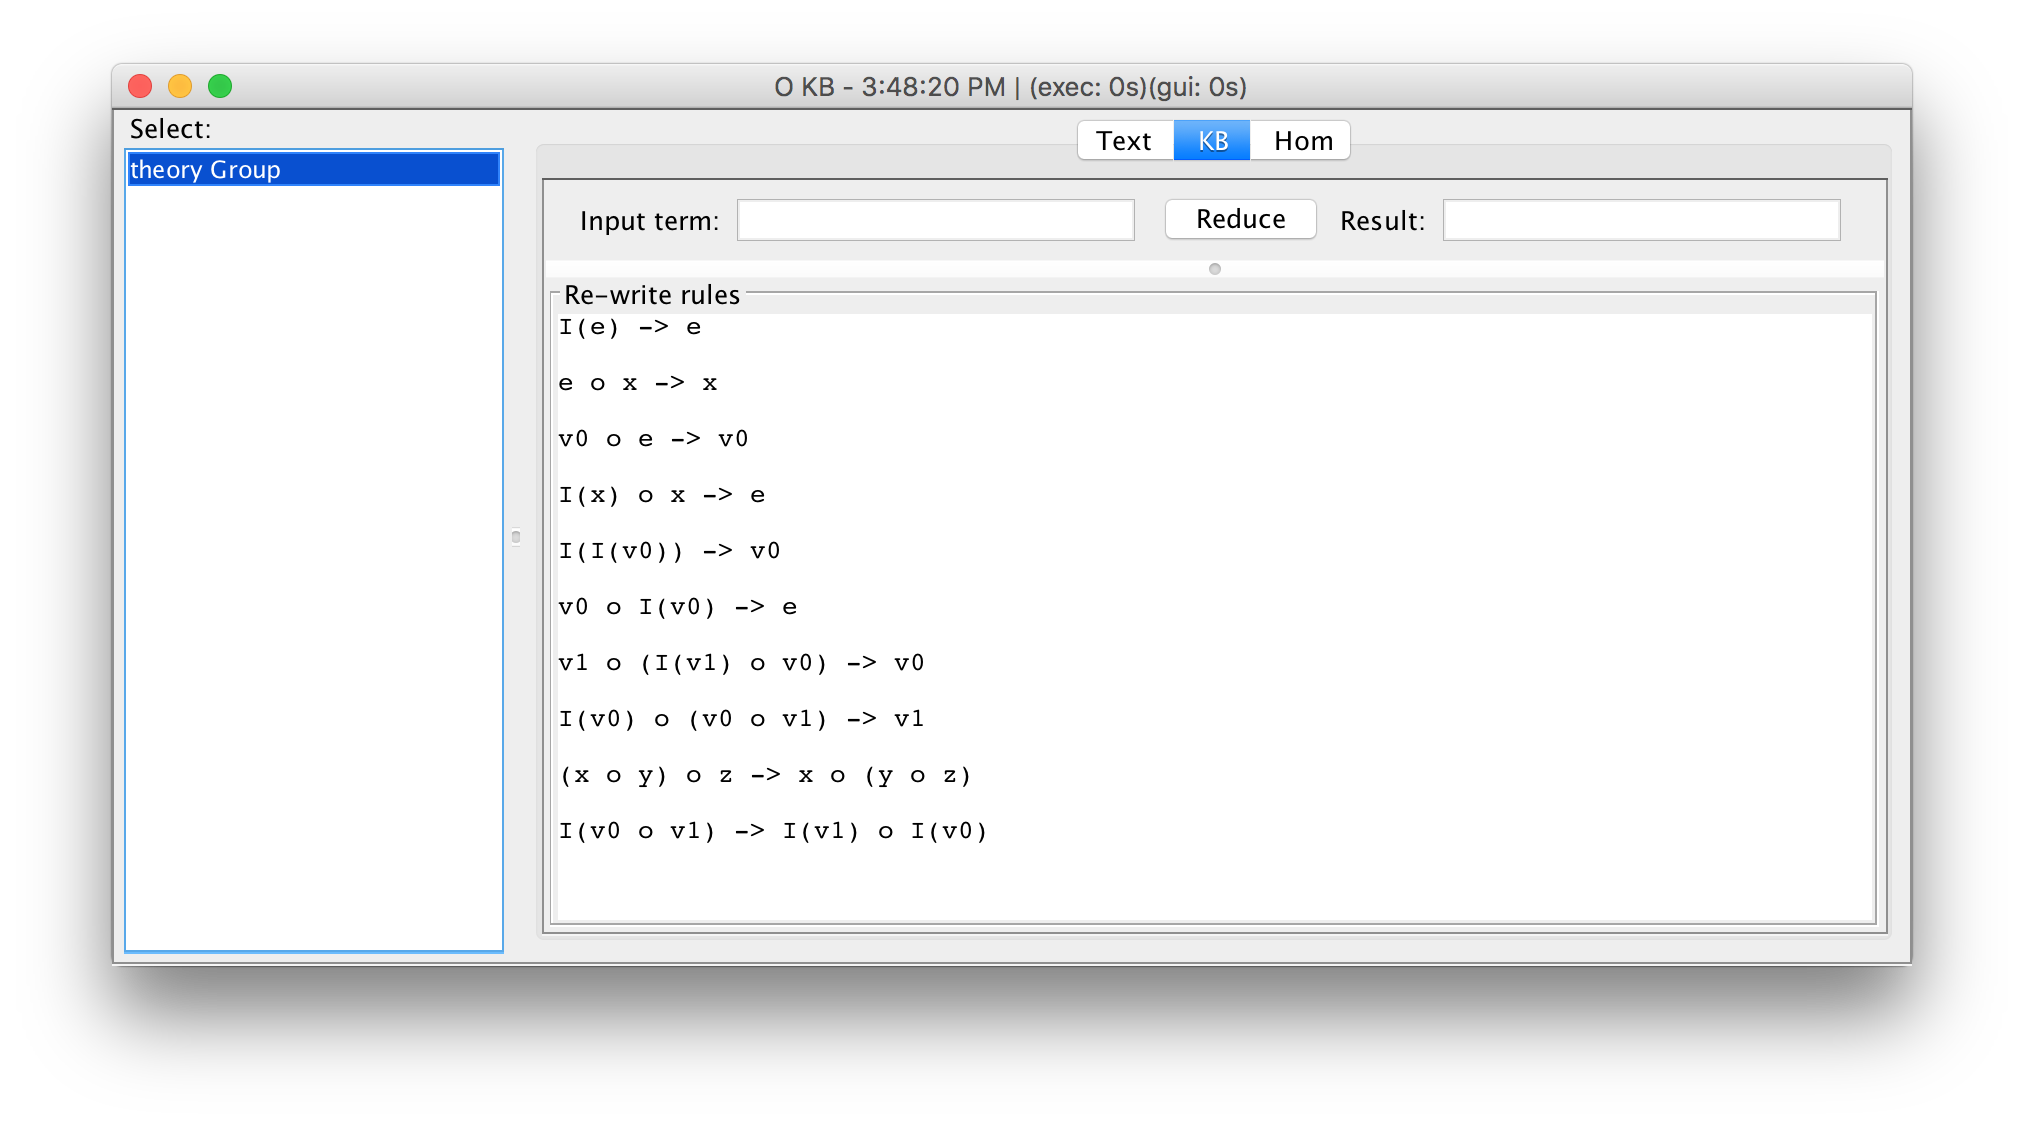
\includegraphics[width=6in]{group1}
\end{center}

The OPL IDE performed ``Knuth-Bendix completion'' on this theory: it transformed the three input equations into ten {\it re-write rules}.  (Note that the viewer will pretty-print the rewrite rules by writing function symbols with arity 2 in infix notation, and omitting universal quantifiers.) To decide the equality of two (possibly open) terms in the original theory, the terms are reduced to normal forms using these re-write rules; then, the normal forms are compared for syntactic equality.  The KB tab can be used to compute such normal forms.

Note that Knuth-Bendix completion is not computable; if completion does not terminate within a certain amount of time (specified in the OPL options menu), an exception is thrown.  In addition, completion is sensitive to the {\it precedence} of the function symbols; applications of functions with higher precedence are re-written into applications of functions with lower precedence.  In this example, OPL uses a built-in precedence of $I > o > e$, but this can be overridden by the user by using $@$ annotations, for example, to set $o > I > e$, write:
\begin{verbatim}
	e@0 : S,
	I@1 : S -> S,
	o@2 : S,S -> S;
\end{verbatim}	
This precedence does not result in a complete re-write system, and the IDE will throw an error.  Note that precedences must be unique; it is not possible to give two function symbols the same precedence.  Finally, note that the $()$ symbols can be omitted on 0-ary constants, that it is permissible to write e.g., {\tt forall x:Nat} rather than just {\tt forall x} in an equation, and that {\tt forall}s may be omitted when empty.

\subsection{Set-valued Models}

A (finite, set-valued) {\it model} of a theory assigns a set to each sort and a function of appropriate arity to each function symbol.  Continuing with the group example, we can specify a trivial group as follows:
\begin{verbatim}
TrivialGroup = model {
	sorts S -> {x};
	symbols e -> { ((),x) },
		   I -> { ((x),x) },
		   o -> { ((x,x),x) };
} : Group 
\end{verbatim}
This model will be rendered in the viewer in tabular form:
\begin{center}
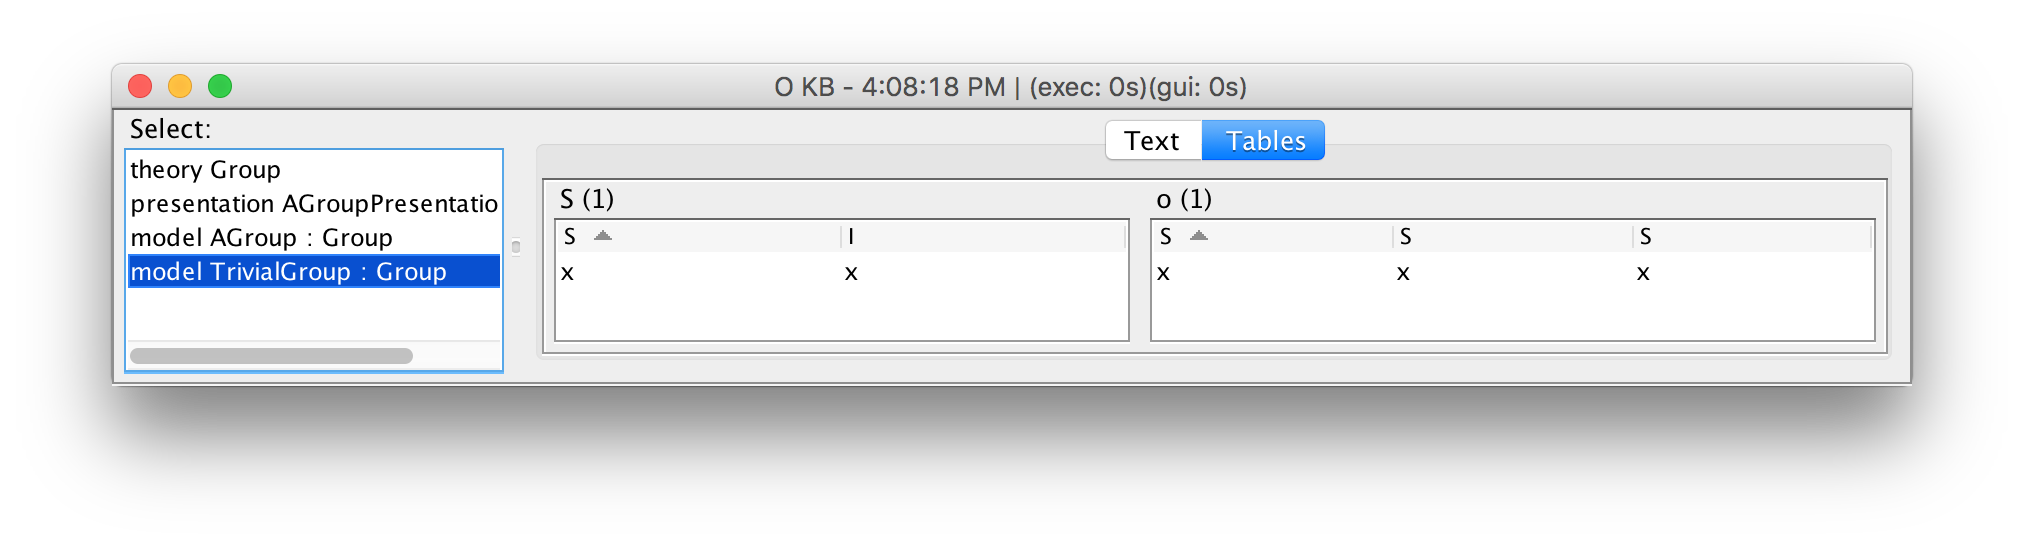
\includegraphics[width=6in]{group2}
\end{center}
Of course, we can replace ``x'' by any other string and still have a trivial group.

\subsection{Presentations}
A (finite) {\it presentation} on a theory is a set of generators (0-ary function symbols) and equations extending the underlying theory.  Presentations can be {\it saturated} into so-called term, or initial, models; these are models built from the syntax of the presentation.  Models, in turn, can be {\it unsaturated} into presentations (although in general, a presentation will not be syntactically equal to the unsaturation of its saturation).  Note that presentations may saturate into infinite models, if so, the IDE throws an error.  Continuing with the group example, we can define a group presentation on one generator as follows:
\begin{verbatim}
AGroupPresentation = presentation {
	generators g : S;
	equations o(g, o(g, g)) = g;
} : Group
AGroup = saturate AGroupPresentation
AGroupPresentationAgain = unsaturate AGroup
AGroupAgain = saturate AGroupPresentationAgain
\end{verbatim}
\begin{center}
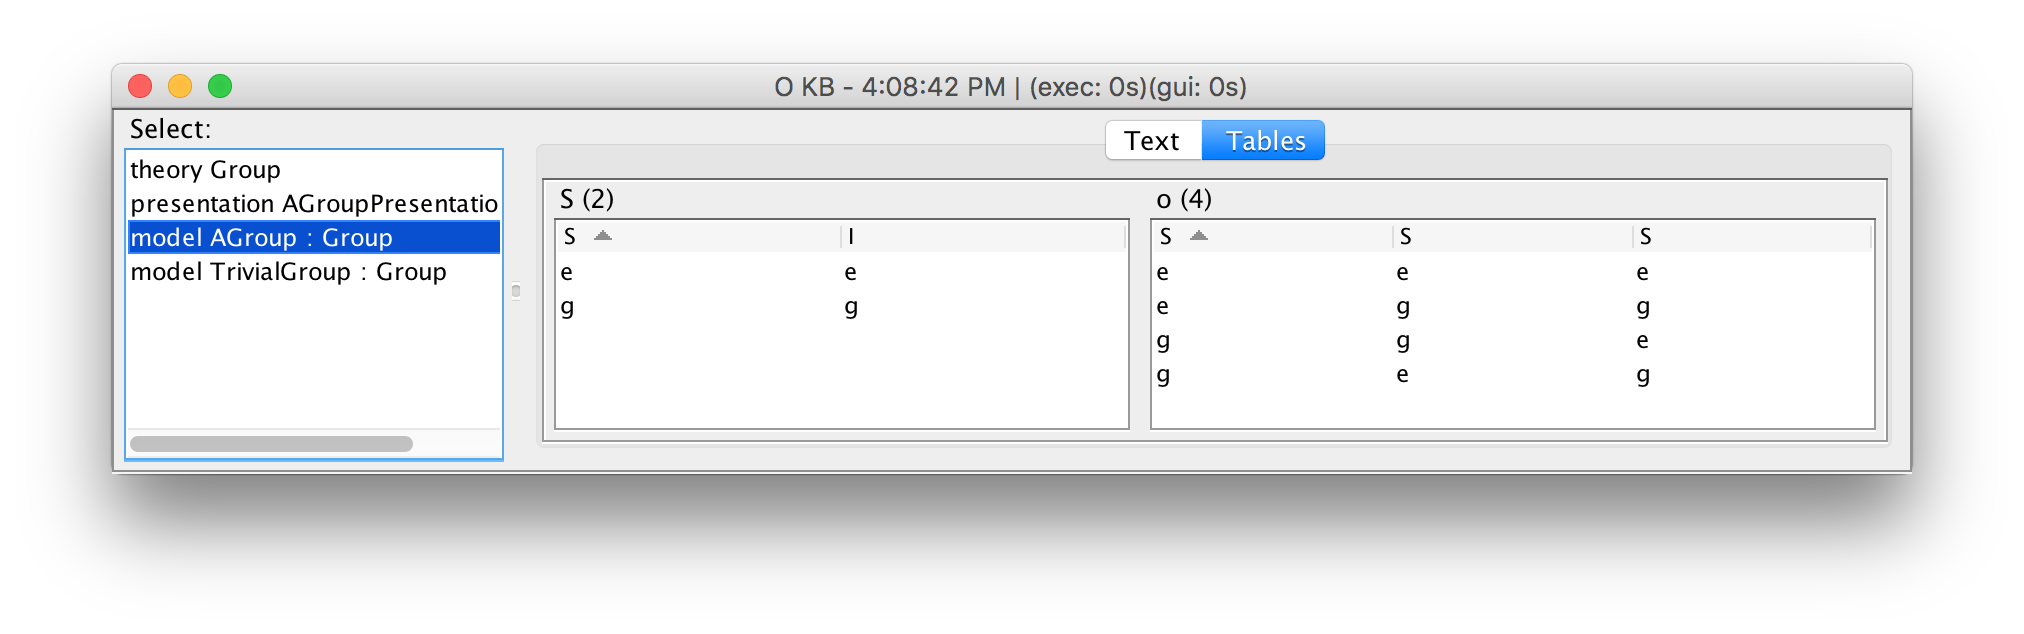
\includegraphics[width=6in]{group3}
\end{center}
The ``Hom'' tab of a presentation in the viewer can be used to find the set of terms of a given type (so-called ``hom sets'') in the saturated model.  For example, entering a blank source and a target of $S$ in $AGroupPresentation$ displays two terms, $e$ and $g$.  In general, when the source is not empty, the resulting terms will contain variables.  In the group example, the hom sets with non-empty sources are infinite and cannot be displayed; the hom set $S \to S$ contains, for example, $y$, $y \circ y$, $y \circ y \circ y$, etc, where $y : S$ is a variable.  

\subsection{Transforms}
A transformation $h : I \to J$ between two set-valued models on the same theory is specified using the {\tt transform} keyword and, for each sort $x$, a function $I(x) \to J(x)$, subject to certain naturality conditions.  See ``O Mod4'' and ``O Delta'' for examples.  A transform $h' : I' \to J'$ between two presentations is specified using the {\tt transpres} keyboard and, for each sort $x$, and for each generator $g \in I'(x)$, a (closed) term of sort $x$ in $I'(x)$.  See ``O Sigma'' for an example.
 
\subsection{Javascript-valued models}
In addition to set-valued models, described above, OPL also includes Javascript-valued models.  Load the ``O JS'' example, and observe that the equations for $T$ do not fully specify the intended behavior of the reverse function:
\begin{verbatim}
T = theory {
	sorts 
		Int, String;
	symbols 
		zero : Int,
		succ, pred : Int -> Int,
		length : String -> Int,
		reverse : String -> String,
		append : String, String -> String,
		print : Int -> String;
	equations	
		forall x. pred(succ(x)) = x,
		forall x. succ(pred(x)) = x,
		forall x. length(x) = length(reverse(x));
}

M = javascript {
	symbols
		_preamble -> "javax.swing.JOptionPane.showMessageDialog(null, \"hello\")",
		zero -> "return 0",
		succ -> "return (input[0] + 1)",
		pred -> "return (input[0] - 1)",
		length -> "return input[0].length",
		reverse -> "return input[0].split('').reverse().join('')",
		append -> "return input[0].concat(input[1])",
		print -> "return input[0].toString()";
} : T

z = eval M zero()
sz = eval M succ(zero())
ssz = eval M succ(succ(zero()))
pssz = eval M pred(succ(succ(zero())))

test1 = eval M append(print(succ(zero())), print(zero()))
rev_test1 = eval M reverse(append(print(succ(zero())), print(zero())))
len_test1 = eval M length(reverse(append(print(succ(zero())), print(zero()))))
\end{verbatim}

Here, $M$ is a javascript valued model on the theory $T$ that does fully specify the behavior of $append$; to specify a javascript valued model is to specify a javascript expression for each function symbol.  The input to each function is represented as a tuple variable named $input$, so for example the append function uses $input[0]$ and $input[1]$ respectively to access its two inputs.  Each javascript model can also contain a preamble, which will execute before any other javascript functions execute; here, the preamble displays a dialog box.  The $eval$ keyword evaluates a term in  a javascript model.  We see, for example, that $test1$ evaluates to a javascript 10.  Note that there is no notion of a transform between javascript models.  Javascript models will be discussed further in the next section.  The javascript expressions are evaluated using Java 8's built in Nashorn engine, and hence the javascript expressions can interact with the VM in which OPL is running, for example by calling java classes.  If $x = \ldots$ is a declaration in an OPL program, then the variable $x$, when invoked in a javascript expression, will return the internal OPL java object representing $x$, thereby allowing reflective capabilities.

\subsection{Mappings}

A {\it mapping} $F : S \to T$ between two theories is a function mapping each sort in $S$ to a sort in $T$, and each symbol $f : s_1, \ldots, s_n \to s$ in $S$ to a term-in-context $v_1 : F(s_1), \ldots, v_n : F(S_n) \vdash F(f) : F(s)$ in $T$, such that if $P = Q$ holds in $S$, then $F(P) = F(Q)$ holds in $T$.  Mappings are demonstrated in the next two subsections.

\subsection{Delta}

If $F : S \to T$ is a mapping, and $J$ is a model on $T$, then $\Delta_F(J)$ is a model on $S$.  This is illustrated in the ``O Delta'' example.
\begin{verbatim}
C = theory {
 	sorts 
		T1, T2, string, int;
 	symbols
		t1_ssn, t1_first, t1_last : T1 -> string,
		t2_first, t2_last : T2 -> string,
		t2_salary : T2 -> int;
 	equations; 
}

D = theory {
 	sorts 
		T, string, int;
 	symbols
		ssn0, first0, last0    : T -> string,
		salary0 : T -> int;
 	equations;
}

F = mapping {
 	sorts 
		T1 -> T,
		T2 -> T,
		string -> string,
		int -> int;
 	symbols
		t1_ssn    -> forall x:T. ssn0(x),
		t1_first  -> forall x:T. first0(x),
		t2_first  -> forall x:T. first0(x),
		t1_last   -> forall x:T. last0(x),
		t2_last   -> forall x:T. last0(x),
		t2_salary -> forall x:T. salary0(x);
} : C -> D

J = model {
	sorts 
		T -> { XF667, XF891, XF221 },
		string -> { "115-234", "112-988", "198-887", Bob, Sue, Alice, Smith, Jones },
		int -> { 250, 100, 300 };
 	symbols
		ssn0    -> { ((XF667), "115-234"),((XF891),"112-988"),((XF221),"198-887") },
		first0  -> { ((XF667),Bob),((XF891),Sue),((XF221),Alice) },
		last0   -> { ((XF667),Smith),((XF891),Smith),((XF221),Jones) },
		salary0 -> { ((XF667),250),((XF891),300),((XF221),100) };
} : D 

deltaFJ = delta F J
\end{verbatim}

$\Delta$ can also be applied to transforms: if $h : I \to J$, then $\Delta_F(h) : \Delta_F(I) \to \Delta_F(J)$.  This functionality is also demonstrated in ``O Delta''.

\subsection{Sigma}
If $F : S \to T$ is a mapping, and $I$ is a presentation on $S$, then $\Sigma_F(I)$ is a presentation on $T$.  This is illustrated in the ``O Sigma'' example.
\begin{verbatim}
C = theory {
	sorts 
		Amphibian,
		LandAnimal,
		WaterAnimal,
		String;
	symbols
		attA: Amphibian -> String, 
		attL: LandAnimal -> String, 
		attW: WaterAnimal -> String,
		IsAL: Amphibian -> LandAnimal,
		IsAW: Amphibian -> WaterAnimal;
	equations;
}

I0= presentation {
	generators 
		a1, a2 : Amphibian,
		l1, l2, l3, l4, l5 : LandAnimal,
		w1, w2, w3, w4 : WaterAnimal,
		gecko, frog, human, cow, horse, dolphin, fish : String;
	equations
		 attA(a1) = gecko,  attA(a2) = frog,
		 attL(l1) = gecko,  attL(l2) = frog, 
		 attL(l3) = human,  attL(l4) = cow, 
		 attL(l5) = horse,  attW(w1) = fish, 
		 attW(w2) = gecko,  attW(w3) = frog, 
		 attW(w4) = dolphin,  IsAL(a1) = l1, 
		 IsAL(a2) = l2,  IsAW(a1) = w2,  IsAW(a2) = w3; 
} : C

D = theory {
	sorts 
		yAmphibian,
		yLandAnimal,
		yWaterAnimal,
		yAnimal,
		String;
	symbols
		yattA:yAmphibian->String, 
		yattL:yLandAnimal->String, 
		yattW:yWaterAnimal->String,
		yIsAL:yAmphibian->yLandAnimal,
		yIsAW:yAmphibian->yWaterAnimal,
		yIsALL:yLandAnimal->yAnimal,
		yIsAWW:yWaterAnimal->yAnimal;
	equations
		forall x. yIsALL(yIsAL(x)) = yIsAWW(yIsAW(x));
}

F = mapping {
	sorts 
		Amphibian->yAmphibian,
		LandAnimal->yLandAnimal,
		WaterAnimal->yWaterAnimal,
		String -> String;
	symbols
		attA -> forall x. yattA(x), 
		attL -> forall x. yattL(x), 
		attW -> forall x. yattW(x),
		IsAL -> forall x. yIsAL(x),
		IsAW -> forall x. yIsAW(x);
} : C -> D

J = sigma F I0
\end{verbatim}

$\Sigma$ can also be applied to transforms: if $h : I \to J$, then $\Sigma_F(h) : \Sigma_F(I) \to \Sigma_F(J)$.  This functionality is also demonstrated in ``O Sigma''.

\subsection{Pi}

OPL does not expose a $\Pi$ primitive.  Rather, $\Pi$ must be expressed as a query, as discussed in the next section.

\section{Typed OPL}

Like FQL and FPQL, OPL can distinguish between sorts that are ``types'' and sorts that are ``entities'', and this distinction is useful for functorial data migration.

\subsection{Schemas}

An OPL {\it schema} is a pair of a {\it theory} and a set of sorts in the theory that are to be treated as {\it entities}; sorts that are not entities are called {\it types}.  Open the ``O Ty Emp'' example.
\begin{verbatim}
S0 = theory { 
 sorts
 	Employee, Department, string, nat;
 symbols
 	Al, Akin, Bob, Bo, Carl, Cork, Dan, Dunn, Math, CS : string,
 	zero 	: nat,
 	succ		: nat -> nat,
 	plus		: nat, nat -> nat,
 	print	: nat -> string,
 	length 	: string -> nat,
 	reverse 	: string -> string,
 	append	: string, string -> string,
     first, last, middle 	: Employee -> string,
     age		: Employee -> nat,
     name 	: Department -> string,
	manager   : Employee -> Employee,
	worksIn   : Employee -> Department,
	secretary : Department -> Employee;
 equations  
 	forall x. plus(x,zero) = x,
 	forall x, y. plus(succ(x),y) = succ(plus(x,y)),
 	forall x. reverse(reverse(x)) = x,
 	forall x. length(x) = length(reverse(x)),
 	forall x, y. length(append(x,y)) = plus(length(x),length(y)),
  	forall x. worksIn(manager(x)) = worksIn(x),
  	forall x. worksIn(secretary(x)) = x;
  //	forall x. manager(manager(x)) = manager(x); can finitize at instance level 
}

S = schema {
	entities
		Employee, Department;	
} : S0

E = entities S
A = attributes S
T = types S
EA = entitiesAndAttributes S
\end{verbatim}

Here, the schema $S$ marks $Employee$ and $Department$ as the entities in theory $S0$.  To be a valid schema, all function symbols from entities must be unary, and there must be no function symbols from types to entities.  Functions between entities are called {\it foreign keys}, and functions from entities to types are called {\it attributes}.  The theory $T$ divides naturally into other theories: an {\it entity side}, consisting of only entities and foreign keys, a {\it type side}, consisting of only types and associated functions, a {\it attribute side} (not typically used), and a combination of the entity and attribute side.   

\subsection{Instances}

An OPL {\it instance} is a combination of a schema, a presentation on that schema, and an (optional) javascript model on the schema's type side.  Use the keyword {\tt none} to specify that a javascript model is not used.  The viewer for the instance displays the saturation of the entity and attribute part of the presentation:

\begin{verbatim}
I0 = presentation {
	generators a, b, c : Employee, 
	           m, s : Department;
	equations first(a) = Al, 
			first(b) = Bob,  last(b) = Bo,
			first(c) = Carl, 
			name(m)  = Math, name(s) = CS,
			age(a) = age(c), //eq of 2 skolems
			last(a) = last(b), //eq 1 skolem, 1 not
			middle(a) = append(first(a),first(b)), //computation
			middle(b) = append(first(a),middle(c)), //partial computation
			manager(a) = b, manager(b) = b, manager(c) = c,
			worksIn(a) = m,  worksIn(b) = m,  worksIn(c) = s,
			secretary(s) = c, secretary(m) = b;
} : S0
I = instance S I0 none
\end{verbatim}

\begin{center}
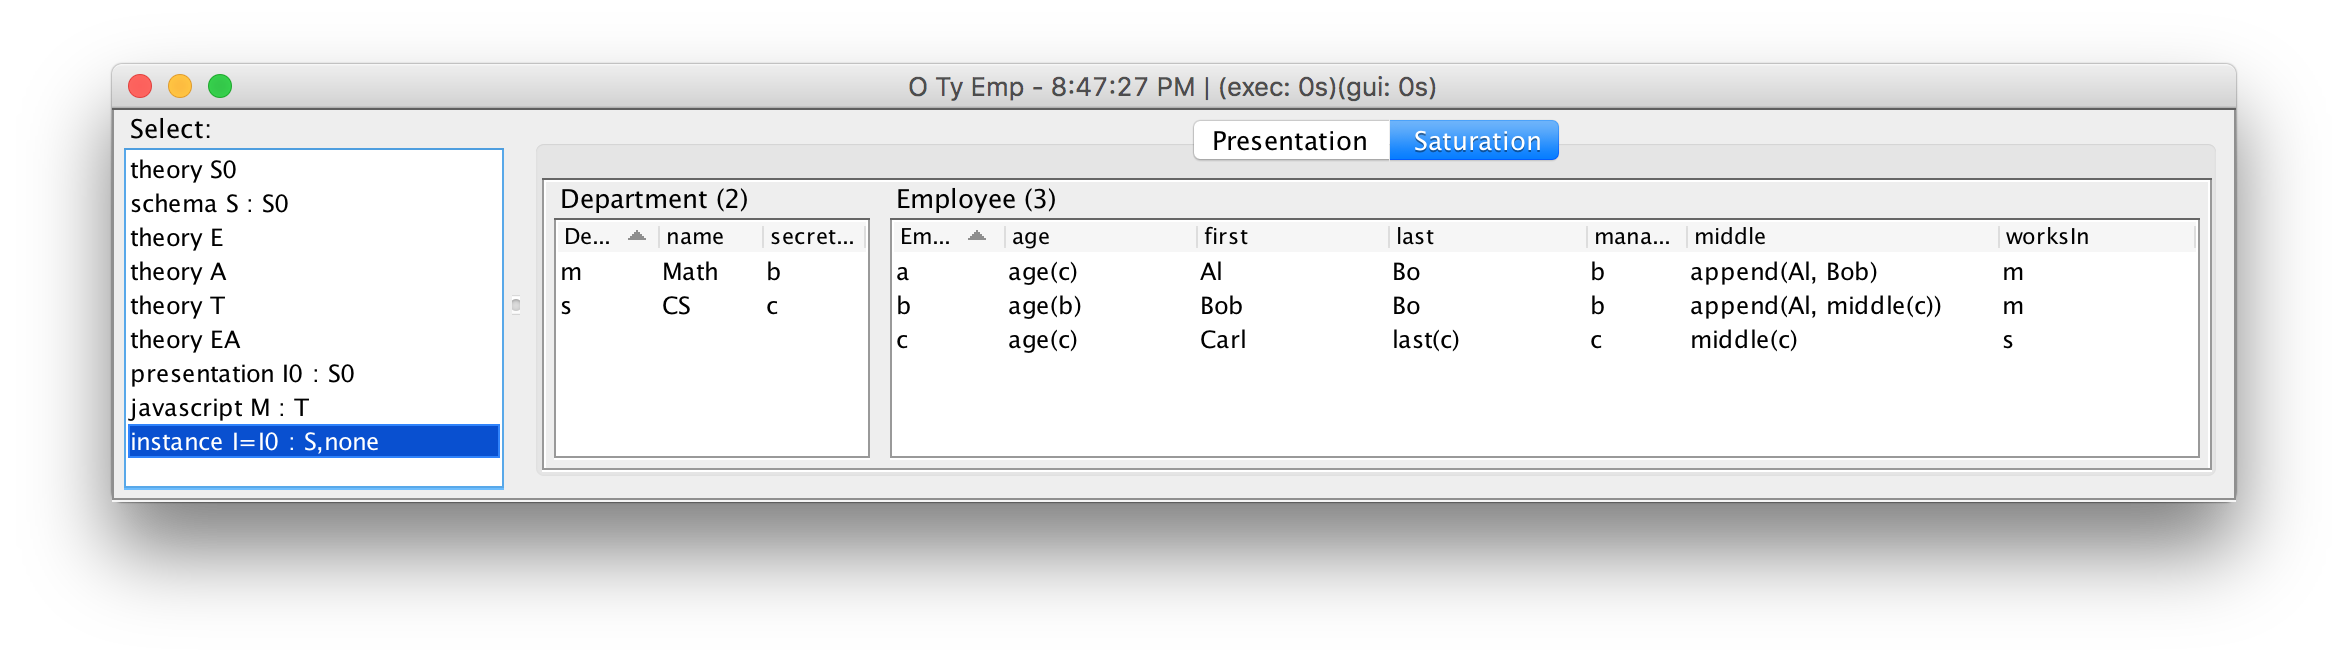
\includegraphics[width=6in]{instance1}
\end{center}

\subsection{Instances that compute}

Continuing with the above example, we may specify a javascript implementation of the type side.  In this case, the viewer will find the image under the type side implementation of the saturation of the entity and attribute part of the presentation. 

\begin{verbatim}
M = javascript {
	symbols
		Al -> "return \"Al\"",
		Akin -> "return \"Akin\"",
		Bob -> "return \"Bob\"",
		Bo -> "return \"Bo\"",
		Carl -> "return \"Carl\"",
		Cork -> "return \"Cork\"",
		Dan -> "return \"Dan\"",
		Dunn -> "return \"Dunn\"",
		Math -> "return \"Math\"",
		CS -> "return \"CS\"",
		zero -> "return 0",
		succ -> "return (input[0] + 1)",
		plus -> "return (input[0] + input[1])",
		length -> "return input[0].length",
		reverse -> "return input[0].split('').reverse().join('')",
		append -> "return input[0].concat(input[1])",
		print -> "return input[0].toString()";
} : T

I = instance S I0 M
\end{verbatim}

\begin{center}
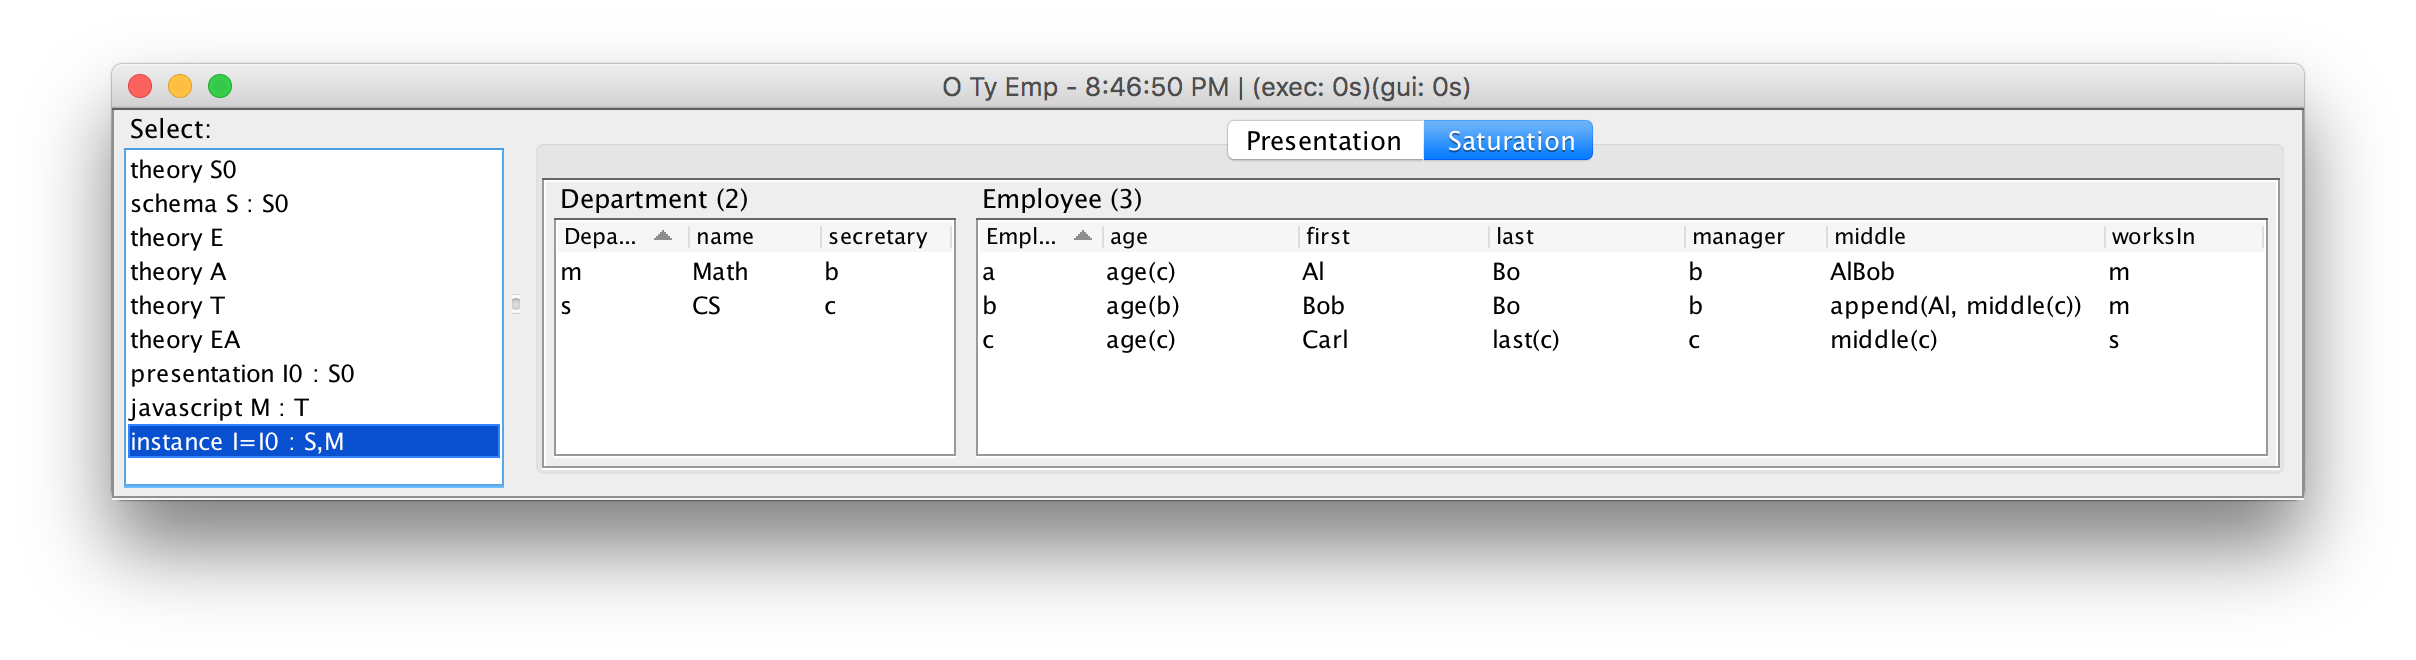
\includegraphics[width=6in]{instance2}
\end{center}

Note that here the javascript strings ``Al'' and ``Bob'' have indeed been appended into ``AlBob.''  We describe several more compelling examples of type side computation.

\subsubsection{Using images and URLs in Instances}

Because OPL's javascript models can invoke arbitrary java code, it is straightforward to embed images in OPL instances.  In the ``O Team Pics" example, images of the OPL team members are fetched from the internet and displayed in the viewer.

\begin{verbatim}
S0 = theory { 
 sorts
 	Person, Image, String;
 symbols
 	cn, dn, rn, pn, jn : String,
 	ci, di, ri, ji : Image,
 	picture : Person -> Image,
 	name : Person -> String;
 equations;
}

S = schema {
	entities Person;	
} : S0

T = types S

I0 = presentation {
	generators c, d, r, p, j : Person;
	equations picture(d) = di, picture(r) = ri, picture(j) = ji, picture(c) = ci,
			name(p) = pn, name(d) = dn, name(r) = rn, name(c) = cn, name(j) = jn;
} : S0

M = javascript {
	symbols
		ri -> "return new javax.swing.JLabel(new javax.swing.ImageIcon(
		new java.net.URL(\"http://wisnesky.net/pic.jpg\")))",						
		di -> "return new javax.swing.JLabel(new javax.swing.ImageIcon(
		new java.net.URL(\"http://math.mit.edu/images/gallery/postdoc/spivak-david.jpg\")))",
		ci -> "return new javax.swing.JLabel(new javax.swing.ImageIcon(
		new java.net.URL(\"http://math.mit.edu/images/gallery/postdoc/vasilakopoulou.png\")))",
		ji -> "return new javax.swing.JLabel(new javax.swing.ImageIcon(
		new java.net.URL(\"http://www.joshuatan.com/wp-content/uploads/2014/11/cropped-IMG-0823.jpg\")))",
		rn -> "return \"Ryan\"",
		dn -> "return \"David\"",
		pn -> "return \"Patrick\"",
		cn -> "return \"Christina\"",
		jn -> "return \"Josh\"";			
} : T

I = instance S I0 M
\end{verbatim}

\begin{center}
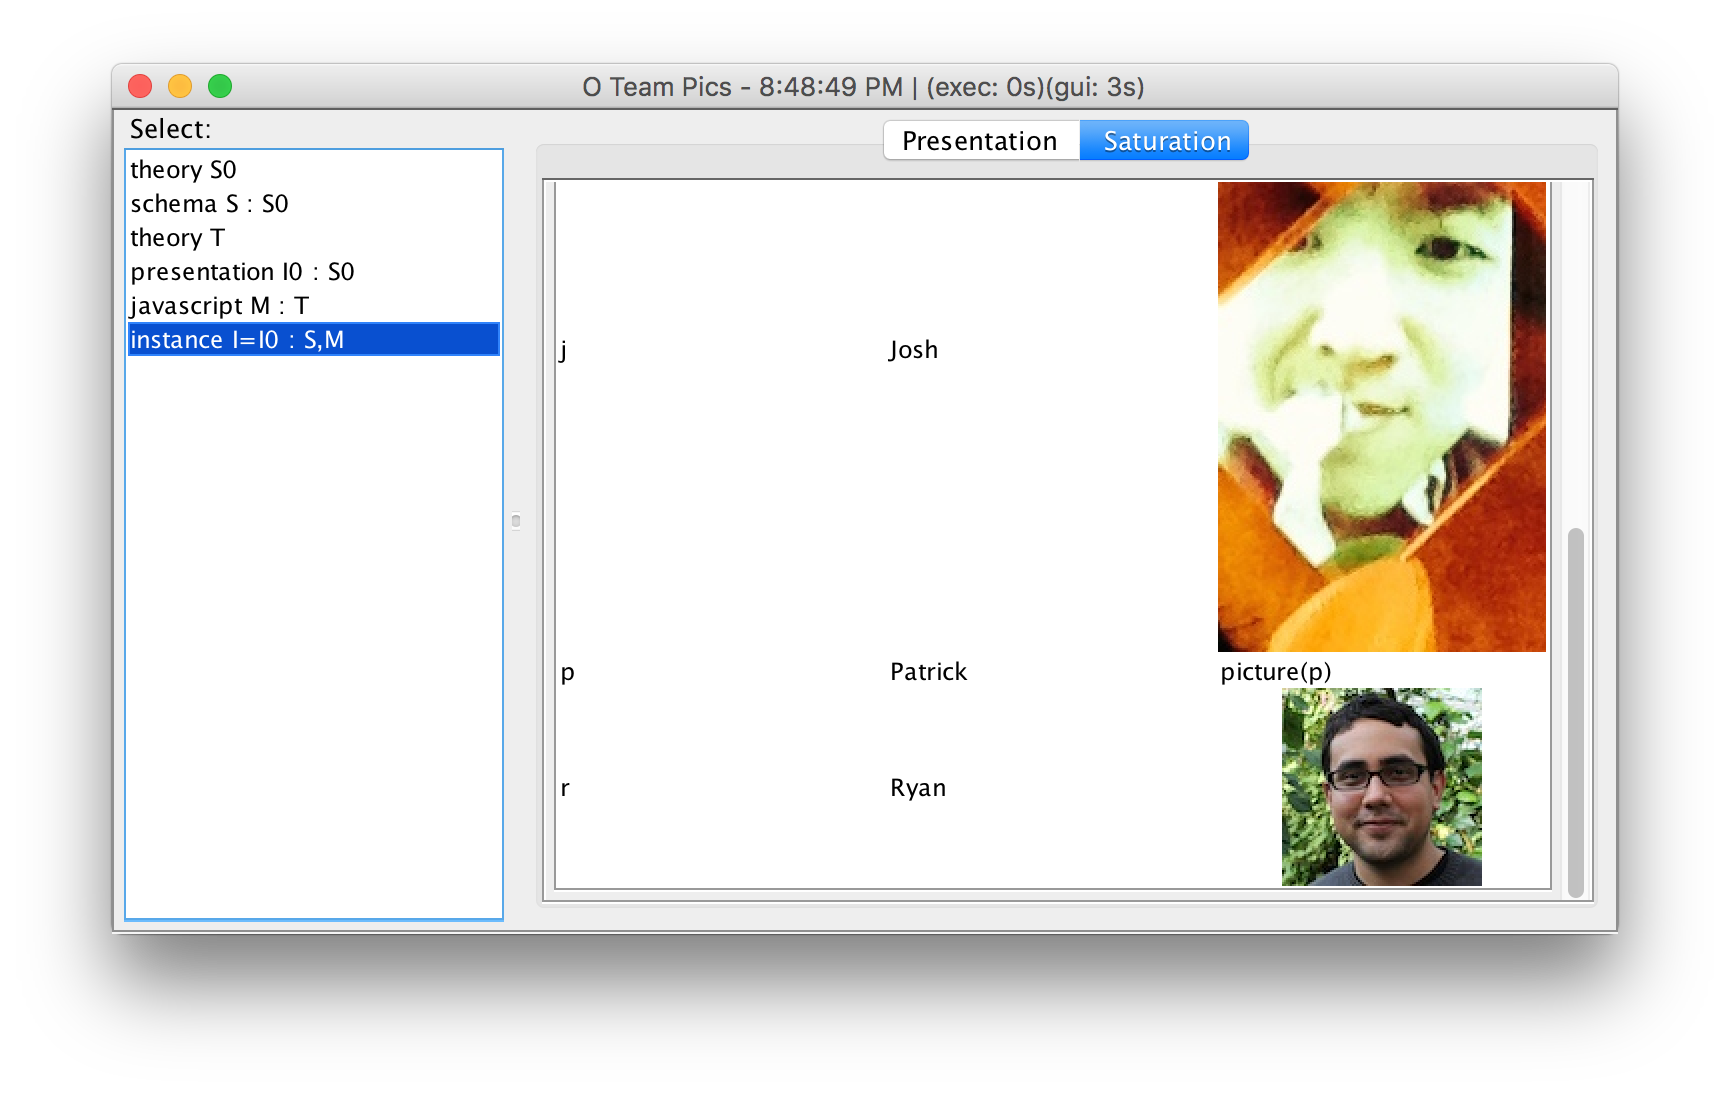
\includegraphics[width=6in]{team}
\end{center}

\subsubsection{Using nested instances in Instances}

In a javascript model, a variable reference such as $x$ will be bound to the FQL artifact corresponding to $x$.  This makes it easy to embed FQL instances inside instances, and to perform aggregations, such as counting the number of rows of an instance.  This is demonstrated in the ``O Nested" example.  Note that to access the nested GUIs for instances in the viewer, it is necessary to double click the nested viewer.

\begin{verbatim}
Ax = theory {
	sorts A1, A2;
	symbols a : A1 -> A2, a1 : A1, a2 : A2;
	equations;
}
A = saturate Ax

Bx = theory {
	sorts B;
	symbols b : B -> B, b1 : B;
	equations forall x. b(x) = x;
}
B = saturate Bx

S0 = theory { 
 sorts
 	M, Model, Int;
 symbols
 	modelOf : M -> Model, 
 	size1 : M -> Int,
 	size2 : Model -> Int,
 	m1, m2 : Model;
 equations
 	forall m. size1(m) = size2(modelOf(m));
}

S = schema {
	entities M;	
} : S0

T = types S

I0 = presentation {
	generators mA, mB : M;
	equations modelOf(mA)=m1, modelOf(mB)=m2;
} : S0

M = javascript {
	symbols
		size2 -> "return input[0].size()",
		m1 -> "return A",
		m2 -> "return B";			
} : T

I = instance S I0 M
\end{verbatim}

\begin{center}
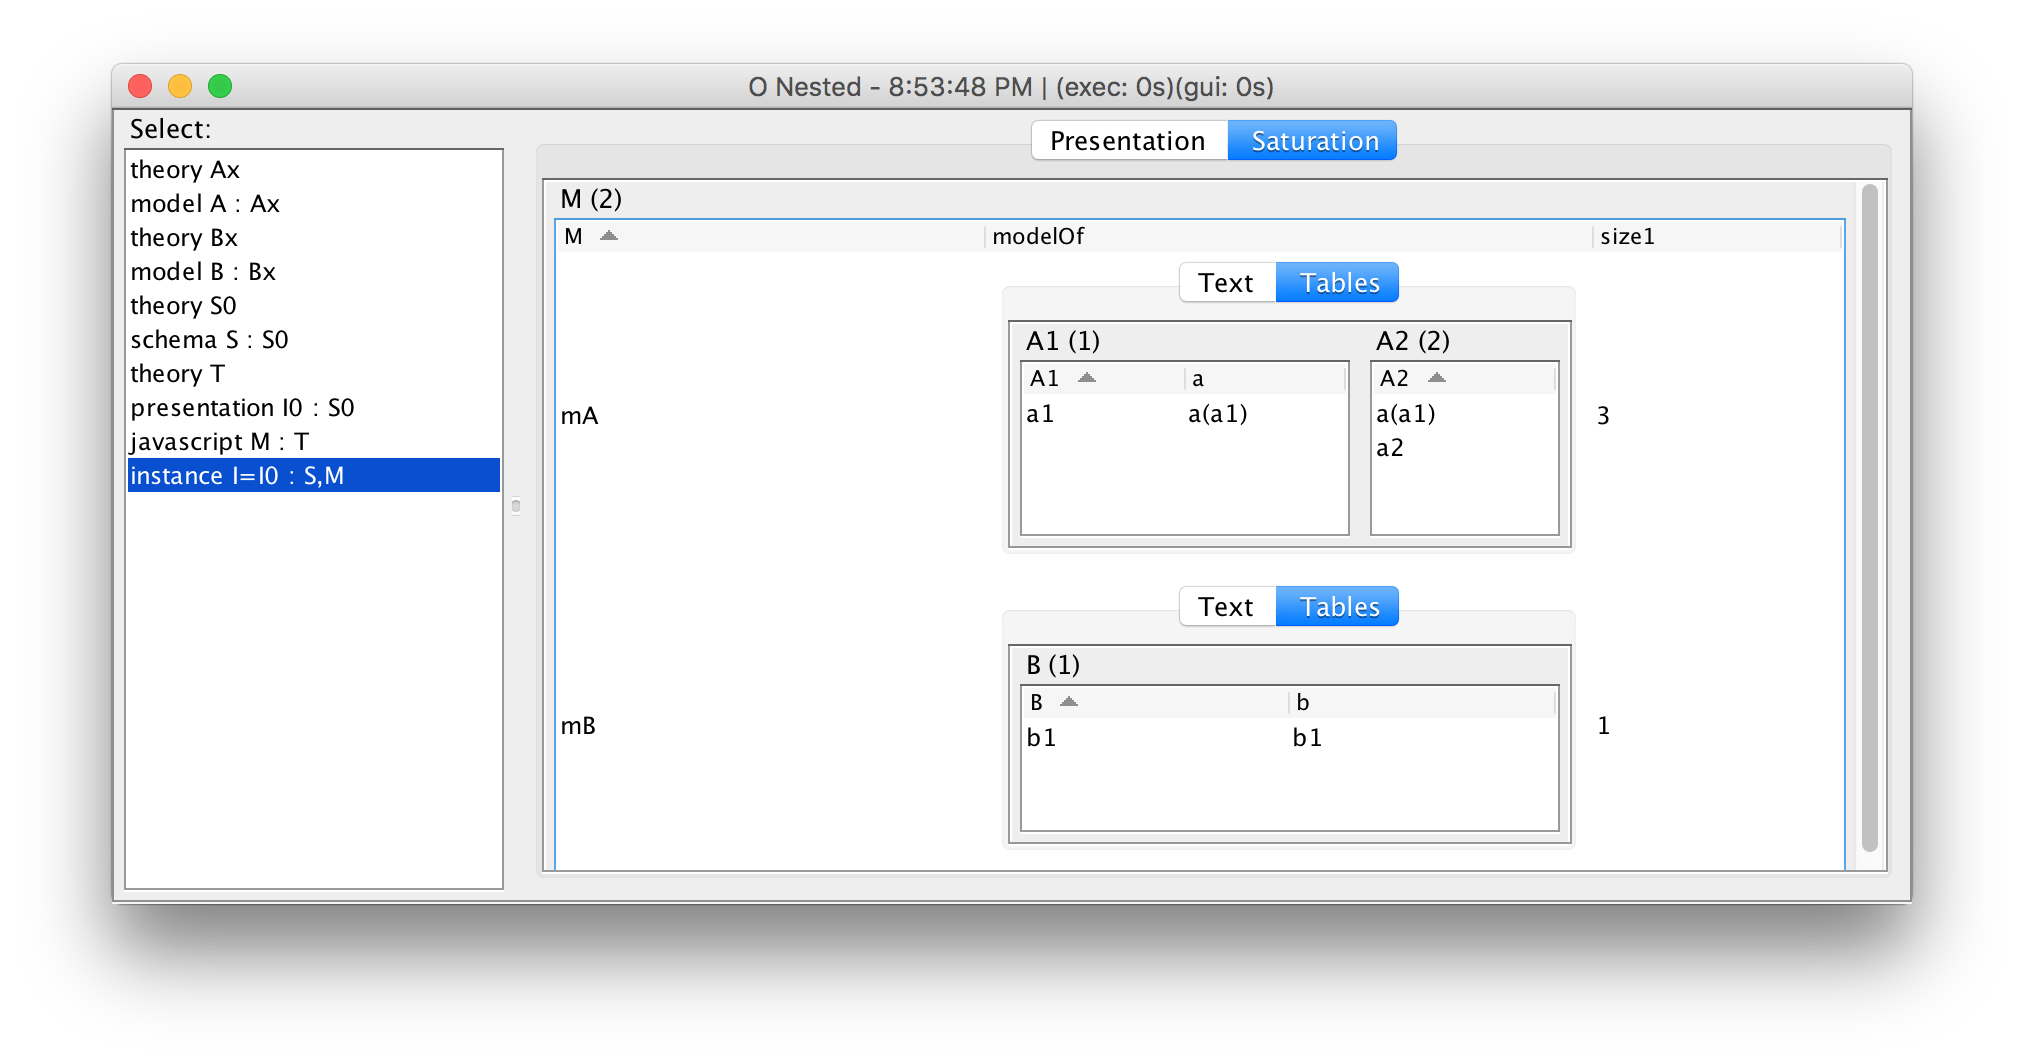
\includegraphics[width=6in]{nested1}
\end{center}

\subsubsection{Using queries in Instances}

As described above, OPL instances can be nested inside of OPL instances.  Additionally, OPL queries may be used to process such nested instances.  In the ``O Nested 2'' example, a $\Delta$ migration is used to process a nested instance.  Note that here it is necessary to use precedence annotations (the $@$ symbols) to force computation to happen.

\begin{verbatim}
Ax = theory {
	sorts A1, A2;
	symbols;
	equations;
}

Bx = theory {
	sorts B;
	symbols b : B;
	equations;
}
B = saturate Bx

F = mapping {
	sorts A1 -> B, A2 -> B;
	symbols;
} : Ax -> Bx 

S0 = theory { 
 sorts
 	M, T1, T2;
 symbols
 	modelOf1@4 : M -> T1, 
 	modelOf2@3 : M -> T2,
 	Q@2 : T2 -> T1,
 	t2@1 : T2;
 equations
 	forall m. modelOf1(m) = Q(modelOf2(m));
}

S = schema {
	entities M;	
} : S0

T = types S

I0 = presentation {
	generators m : M;
	equations modelOf2(m)=t2;
} : S0

M = javascript {
	symbols
		Q -> "return F.delta(input[0])",
		t2 -> "return B";			
} : T

I = instance S I0 M
\end{verbatim} 

\begin{center}
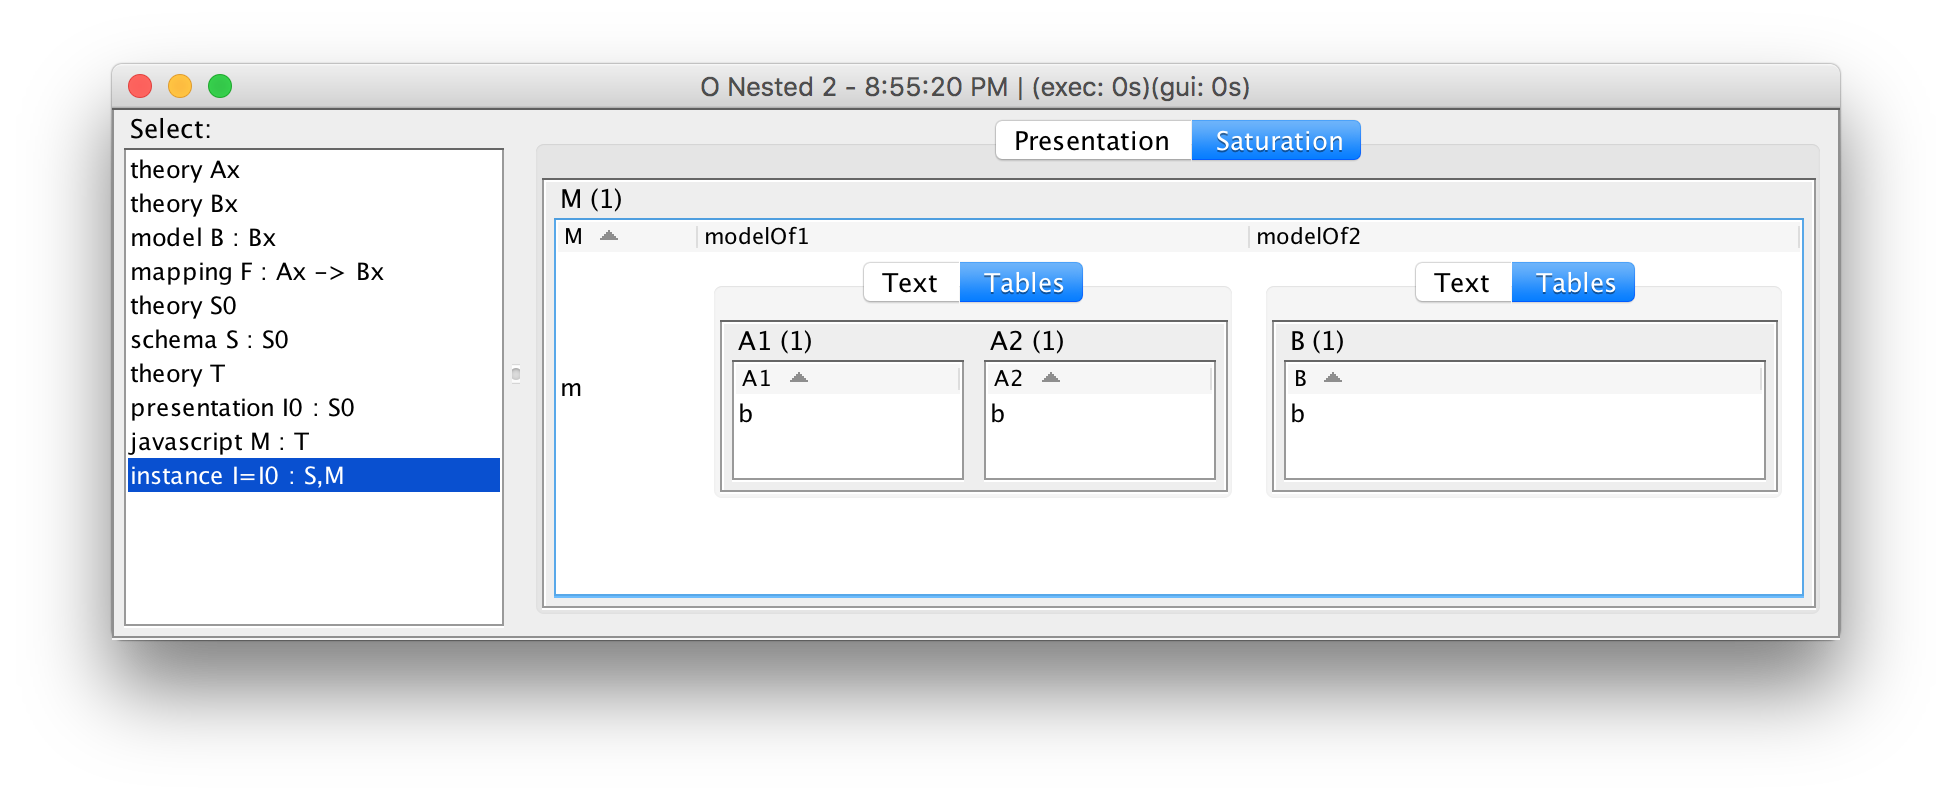
\includegraphics[width=6in]{nested2}
\end{center}

\subsubsection{Using machine learning in Instances}

OPL also supports basic machine learning functionality via a separate FQLML project.  The FQLML project is essentially a bridge between OPL and the Java Machine Learning Library  ({\sf http://java-ml.sourceforge.net/}).  The ``O ML'' project demonstrates this, provided that all necessary libraries are accessible via the IDE's class path.  In this example, people are classified into ``old'' and ``young'' using a nearest neighbor classifier that is trained on half of the input data.  Here precedences annotations (the $@$ symbols) are necessary.

\begin{verbatim}
S0 = theory {
	sorts Person, Nat, String;
	symbols zero@0 : Nat, 
		   succ@1 : Nat -> Nat,
		   old@2, young@3 : String,		   
		   classify@98 : Nat -> String,
   
		   age@99  : Person -> Nat,
		   inputClass@97 : Person -> String,
		   outputClass@100 : Person -> String;
	equations
		forall x. outputClass(x) = classify(age(x));
}

S = schema {
	entities Person;
} : S0

I0 = presentation {
	generators p0, p1, p2, p3, p4, p5, p6, p7 : Person;
	equations age(p0) = 0, age(p1) = 1, age(p2) = 2, age(p3) = 3, 
	          age(p4) = 4, age(p5) = 5, age(p6) = 6, age(p7) = 7,
		     inputClass(p0) = young, inputClass(p1) = young, 
		     inputClass(p6) = old, inputClass(p7) = old;
} : S0
I = instance S I0 none

T = types S


ML = javascript {
      symbols
		_preamble -> "java.lang.Class.forName('fql_lib.opl.ml.MLUtil'); 
var MLUtils = Java.type('fql_lib.opl.ml.MLUtil'); 
var KNNClass = Java.type('net.sf.javaml.classification.KNearestNeighbors'); 
var data = MLUtils.toDataset(I, 'Person', ['age'], 'inputClass'); 
knn = new KNNClass(1); 
knn.buildClassifier(data);",
		zero -> "return 0.0",
		succ -> "return input[0]+1.0",
		old -> "return \"old\"",
		young -> "return \"young\"",
		classify -> "return knn.classify(MLUtils.wrap(input))";
} : T

J = instance S I0 ML
\end{verbatim}

\begin{center}
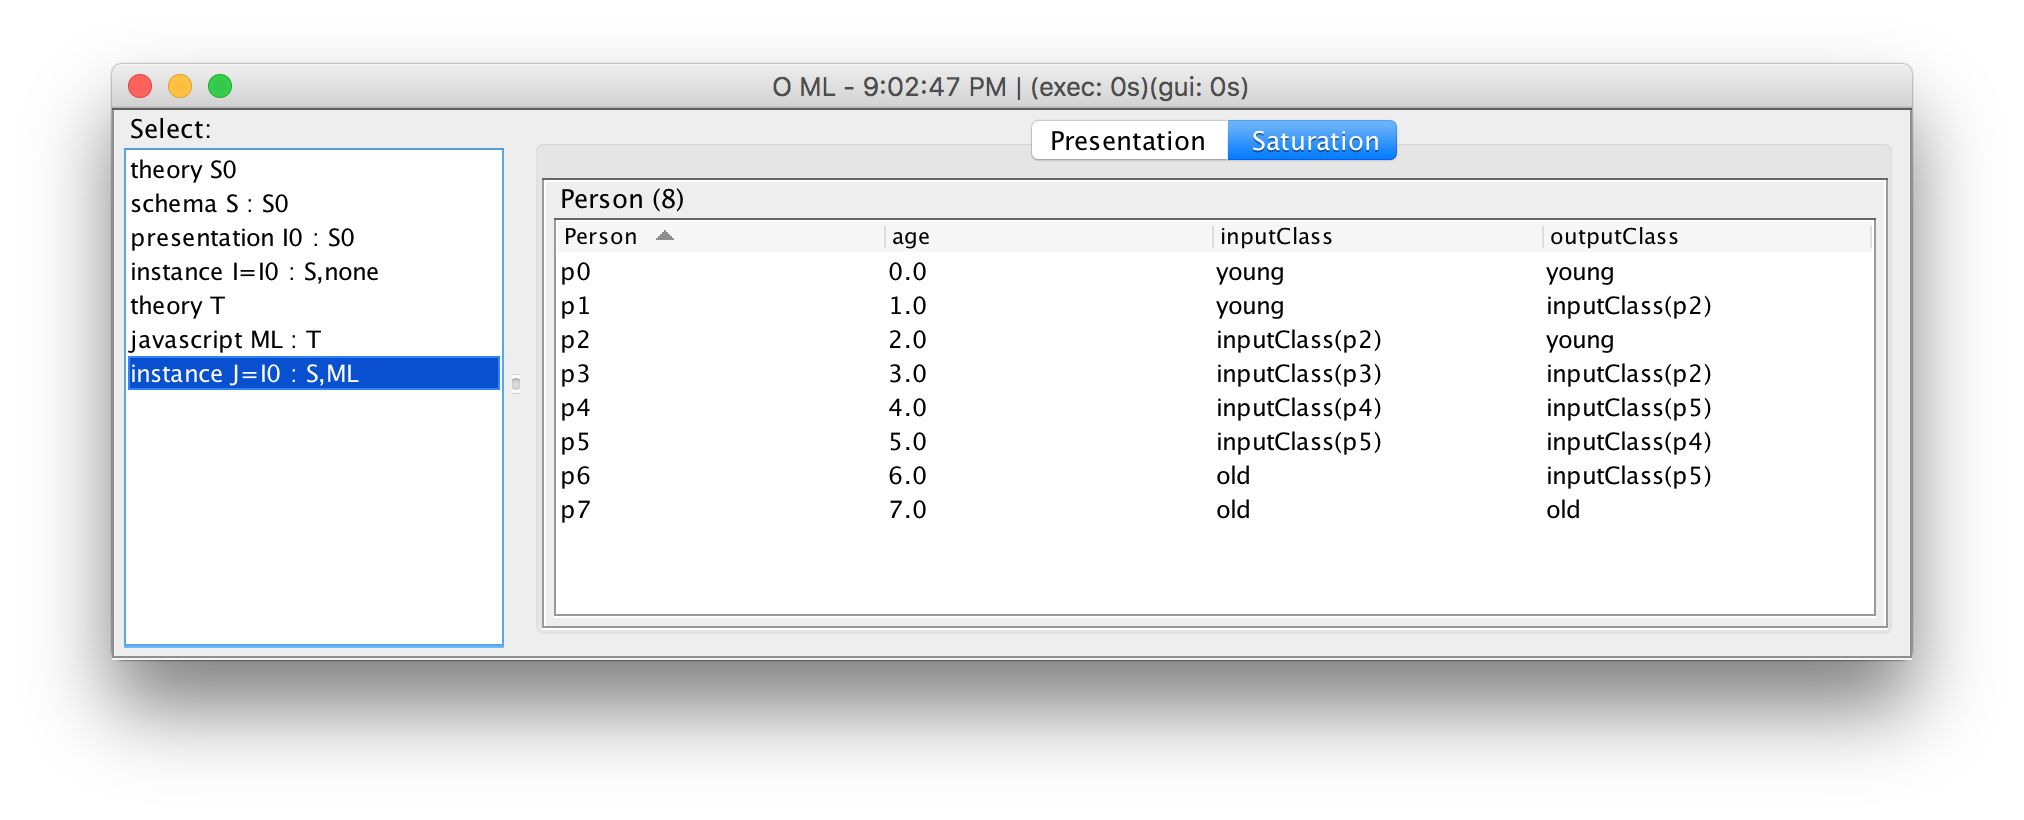
\includegraphics[width=6in]{ml}
\end{center}

\subsubsection{Using 3rd Party Library Code in Instances}

As demonstrated in the above example, to invoke 3rd party java code from javascript in the OPL IDE does not require modifying OPL's source code.  Instead, the required libraries can be loaded dynamically, using Java's {\tt forName} method; in the above example, this is done in the preamble of the javascript model.  For dynamic loading to work, required classes must be on the OPL IDE's class path, and must be fully qualified.  Typically, this is accomplished using a command line option.  For example, to place {\tt mylibrary.jar} on the class path, invoke the IDE using:

\begin{verbatim}
java -cp ``mylibrary.jar'' -jar fql_lib.jar
\end{verbatim}

\subsection{Typed Mappings, Typed Transforms, and Typed Sigma}

If $F : C \to D$ is an OPL mapping, and $S$ is a schema on $C$ and $T$ is a schema on $D$ and $S$ and $T$ have the same type side, then $F$ is also a typed mapping from $S$ to $T$.  To write such a mapping, use the same mapping syntax, except 1) instead of writing $C \to D$, write $S \to T$, and 2) do not give mappings for sorts and symbols that are on the type side.  This same pattern is also true for transforms of presentations (transforms between set-valued models do not make sense in typed OPL).  This is illustrated at the bottom of the ``O Sigma'' example.  Similarly, the $\Sigma$ operation lifts from presentations to instances.  To perform a typed $\Delta$ or a $\Pi$ in OPL it is necessary to use query syntax, defined below.  Query syntax can also be used to define certain $\Sigma$s, those where the mapping is ``union compatible in the sense of Codd''.
 
\subsection{Queries}

The primary query mechanism in OPL is the so-called ``uber-flower'': it presents a data migration of the form $\Sigma_F \circ \Pi_G \circ \Delta_H$, where $F$ is a discrete op-fibration.  A {\it query} $Q : S \to T$, where $S$ and $T$ are schemas containing the same type side, is a collection of {\it blocks}.  Each block contains a {\it label} $l$, a target entity $t$ in $T$, and a {\it flower}, $q$.  The flower $q$ consists of a {\it for} clause, which is a set of variables typed from entities in $T$, a {\it where} clause, which is a collection of equalities between terms built from the variables in the for clause and terms from the source schema, and a {\it return} clause, which describes how to populate the attributes and foreign keys out of $t$ in terms of the variables in the for clause.  This is best illustrated with an example -- the ``O Employees'' example.  In this example, $Q$ is the identity query from $C$ to $C$.

\begin{verbatim}
S = theory { 
 sorts
 	Employee, Department, dom;
 symbols
     first,last: Employee -> dom,
     name 	: Department -> dom,
	manager   : Employee -> Employee,
	worksIn   : Employee -> Department,
	secretary : Department -> Employee;
 equations  
  	forall x. worksIn(manager(x)) = worksIn(x),
  	forall x. worksIn(secretary(x)) = x,
  	forall x. manager(manager(x)) = manager(x);
}

C = schema {
	entities Employee, Department;
} : S

Q = query {
	 qE = {for e:Employee; 
	 	  where; 
	 	  attributes first=first(e), last=last(e); 
	 	  edges manager = {e=manager(e)} : qE, worksIn = {d=worksIn(e)} : qD;} : Employee,
	 qD = {for d:Department; 
	 	  where; 
	 	  attributes name=name(d); 
	 	  edges secretary = {e=secretary(d)} : qE;} : Department
} : C -> C
\end{verbatim}

Here, the $qE$ and $qD$ are labels, and the associated blocks target $Employee$ and $Department$, respectively.  The block for $qE$ says that the populate the $Employee$ table in the target, go through the $Employee$ table in the source; call each such employee $e$.  The first and last name attributes of $e$ in the target should be the same as in the source.  Finally, the manager and worksIn foreign keys for $e$ should be the same in the target as in the source.  Note that for each foreign key, it is required to choose a label $l$, and to give a valuation of the variables in the $l$ FOR clause in terms of variables in the FOR clause of the current block.  Doing so allows the IDE to perform a check that the table populated by this block will not reference any keys in another target table that do not exist.  Significantly more complicated queries are possible, for example:

\begin{verbatim}
Q = query {
	 qE = {for e1:Employee, e2:Employee; 
	 	  where manager(e1)=manager(e2); 
	 	  attributes first=last(e1), last=last(e2); 
	 	  edges manager = {e1=manager(manager(e1)), e2=manager(e1)} : qE, 
	 	        worksIn = {d=worksIn(e1)} : qD;} : Employee,
	 qD = {for d:Department; 
	 	  where; 
	 	  attributes name=name(d); 
	 	  edges secretary = {e1=secretary(d), e2=secretary(d)} : qE;} : Department
} : C -> C
\end{verbatim}

\end{document}


